%short intro
At the LHC, \WZ\ diboson are produced from quark-antiquark initial states at 
leading order (LO) and quark-gluon initial states at next-to-leading order 
(NLO)~\cite{PhysRevD.65.094041}. 
%Figure~\ref{fig:LOdiagrams} shows the LO Feynman diagrams for \WZ production from $q\bar{q}'$ initial states. 
The SM allowed $s$-channel diagram has a triple boson vertex and is sensitive to 
anomalous TGC of gauge bosons.

%FIGURE LO WZ DIAGRAM
% may include 
% figures/sss-inclboson-diboson-wzprod-wz-s-channel.pdf
% figures/sss-inclboson-diboson-wzprod-wz-t-channel.pdf
% figures/sss-inclboson-diboson-wzprod-wz-u-channel.pdf

%\begin{figure}[htbp]
%  \begin{center}
%  \includegraphics[width=0.9\textwidth]{figures/sss-inclboson-diboson-wzprod-wzdiagram.png}
%  \caption{Leading order Feynman diagrams of \WZ production in the dominant 
%  \qqbar\ channel.}
%\label{fig:sss-WZprod-LOdiagrams}
%\end{center}
%\end{figure}

%decay channels


%analysis CMS and ATLAS.
%ATLAS WZ 7 \TeV~\cite{Aad:2012twa}
% - figure from https://atlas.web.cern.ch/Atlas/GROUPS/PHYSICS/PAPERS/STDM-2012-09/
%CMS WZ at 7+8 \TeV (CMS-PAS-SMP-12-006, to be published)
The ATLAS experiment measured the \WZ\ production cross section in the fully 
leptonic decay channel \ll\lnu~\cite{Aad:2012twa} at $\rts = 7\TeV$ and set 
limits on anomalous charged TGC.
%Theoretical calculations
% TBD
% WZ->lllv
%Selections
In this analysis the final states involving electrons or muons are considered signal,
whereas boson decays to tau's are considered as background.  
%Backgrounds
The dominant background sources are \Zboson+jet and \ZZ production, constituting about 40\% of 
the background. The overall signal over background ratio is about 3.7.
%systematics
The dominant systematic uncertainty is from the data-driven estimate of the   
background, where the dominant Z + jets contributes with ($\pm3.8\%$).

% Results at the end
% xsec
The fiducial cross section defined by $\pt^{\mu,e} > 15\GeV$ for the leptons from the \Zboson\ 
 decay, $\pt^{\mu,e} > 15\GeV$ for the lepton from the \Wboson, $|\eta^{\mu,e}|<2.5$, $\pt^\nu>25\GeV$,
 $|m_ll-m_Z| < 10\GeV$, $M_T^W>20GeV$ and $\Delta R> 0.3$ for the three possible $\ell\ell$ pairings. 
The fiducial and total cross sections are compared to the SM expectation at NLO in Table~\ref{tab:sss-WZprod-xsec}.
\begin{table}[htdp]
\begin{center}
\resizebox{\textwidth}{!}{
\begin{tabular}{|c|c|c|c|c|c|}
Experiment & cross section & \rts & measured  & predicted  & reference  \\ \hline
ATLAS & total & 7 GeV & {19 $\pm$ $^{+1.4}_{-1.3}$ (stat.) $^{0.9}$ (syst.) $\pm$ 0.4 (lumi.) pb}  & {17.6  $\pm$ $^{+1.1}_{-1.0}$ pb} & \cite{Aad:2012twa} \\
ATLAS & fiducial & 7 GeV & {92 $\pm$ $^{+7}_{-6}$ (stat.) $^{4}$ (syst.) $\pm$ 2 (lumi.) fb}  & -- & \cite{Aad:2012twa} \\
\end{tabular}
}
\caption{Summary of measured fiducial and total $\WZ$ production cross sections from ATLAS 
at 7 TeV centre-of-mass energies in $\ll\lnu$ final state.}
\end{center}
\label{tab:sss-WZprod-xsec}
\end{table}%


% unfolded spectra
In Figure~\ref{fig:sss-WZprod-ptZ-det} the differential cross section measured in bins of 
$\pt^Z$ is shown, compared to SM prediction and a set of anomalous TGC couplings. 
The normalized $\pt^Z$ spectrum is unfolded and compared to the NLO calculation of \mcatnlo in 
Figure~\ref{fig:sss-WZprod-ptZ-det}, showing good agreement with the SM.


\begin{figure}[htbp]
  \begin{center}
  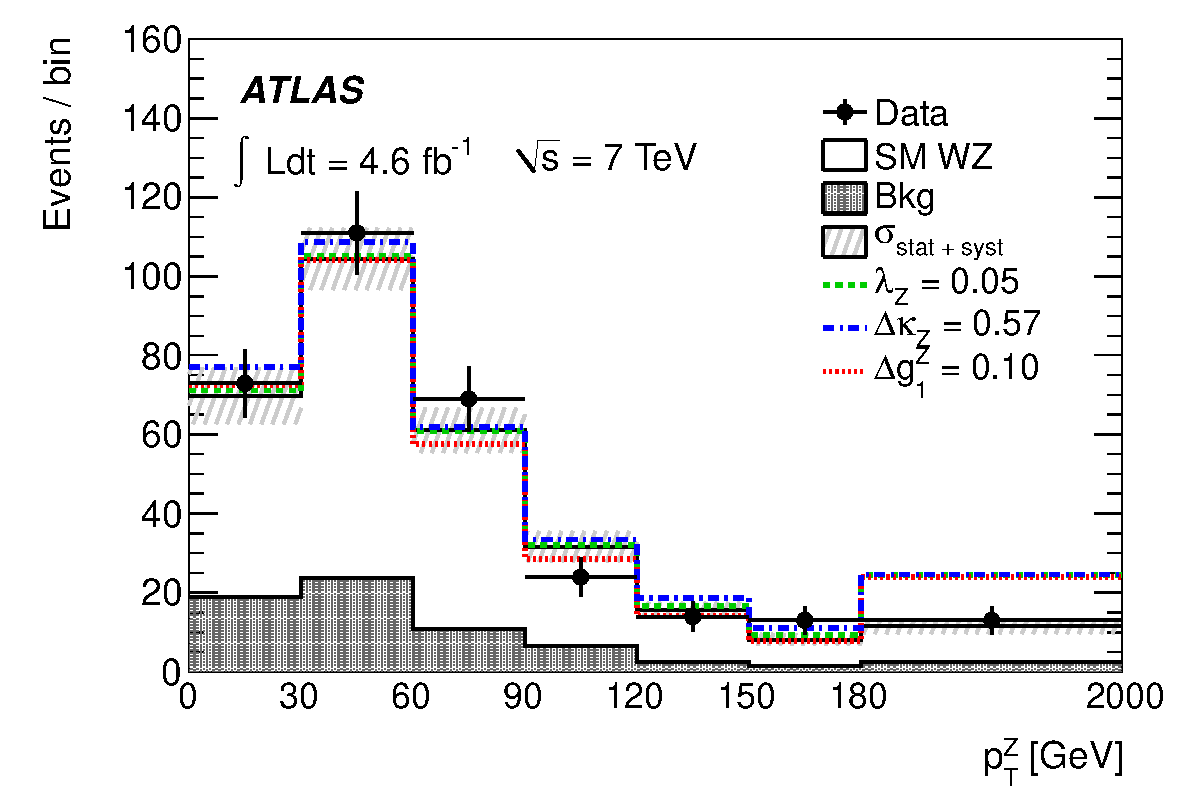
\includegraphics[width=0.45\textwidth]{figures/sss-inclboson-diboson-wzprod-ptZ-det.pdf}
  \caption{ATLAS measurement of the transverse momentum of the \Zboson in \WZ events ($\pt^Z$) compared with the SM prediction at $\rts = 7\TeV$. For illustration calculations for a set of anomalous couplings values are also shown. The full uncertainty contains statistical and systematic uncertainties.}
\label{fig:sss-WZprod-ptZ}
\end{center}
\end{figure}

\begin{figure}[htbp]
  \begin{center}
  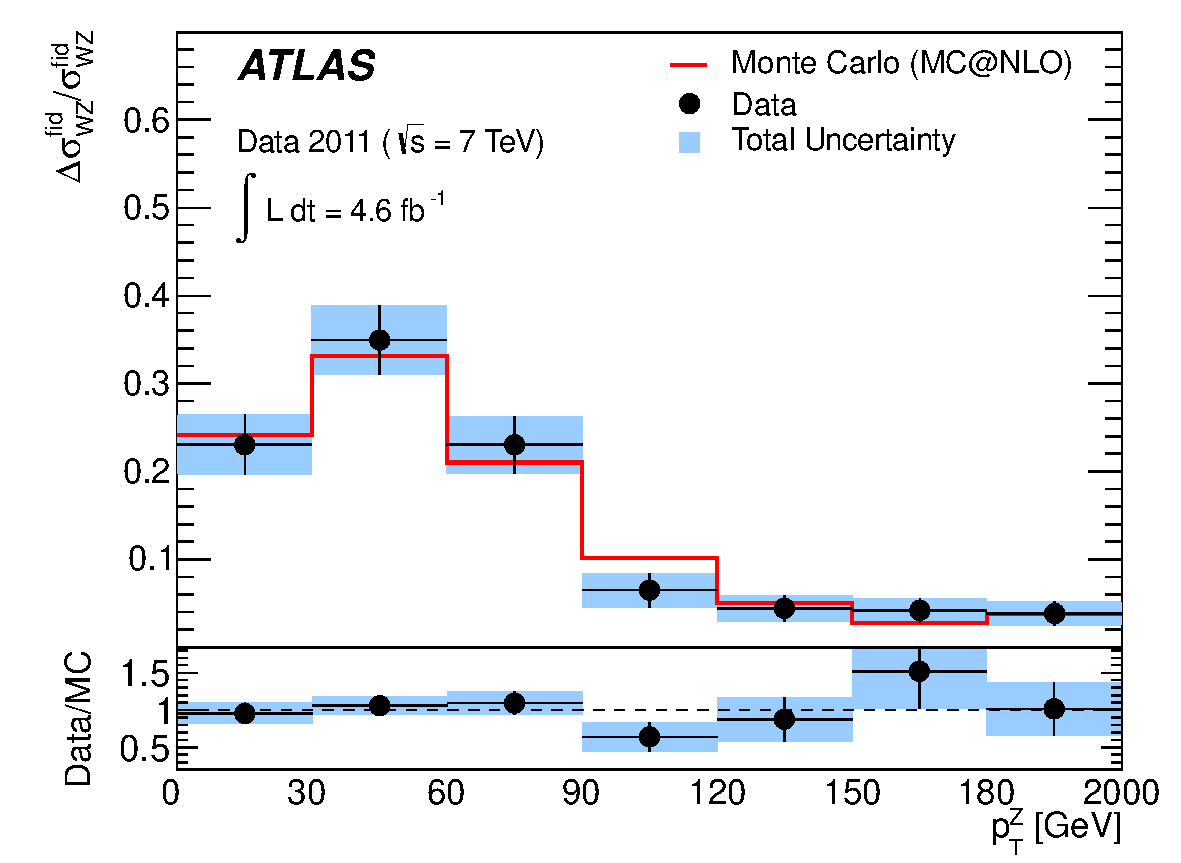
\includegraphics[width=0.45\textwidth]{figures/sss-inclboson-diboson-wzprod-ptZ.pdf}
  \caption{ATLAS measurement of the normalized fiducial cross-sections in bins of $\pt^Z$ compared with the SM prediction at $\rts = 7\TeV$. The full uncertainty contains statistical and systematic uncertainties.}
\label{fig:sss-WZprod-ptZ-det}
\end{center}
\end{figure}


%%%%
% THIS MIGHT GO INTO THE SECTION ON TGC
% aTGC
Limits on the charged ATGC parameters \dkz, \lz\ and \gz\ are extracted from the transverse momentum distribution
of the \Zboson, $\pt^Z$. The ATGC parameter 95\% CL limits are quoted using a form-factor of $\Lambda=2\TeV$ and without a form-factor, and summarized in Table~\ref{tab:sss-WZprod-ATGC}.


\begin{table}\centering
\caption{Expected and observed 95\% CL on 
\dkz, \lz\ and \gz.}
\label{tab:sss-WZprod-ATGC}
\begin{tabular}{cccc}
\hline
& Observed & Observed & Expected \\
& $\Lambda=2$~TeV & no form factor & no form factor\\
\hline
$\gz$ & $[-0.074, 0.133]$ & $[-0.057, 0.093]$ & $[-0.046, 0.080]$ \\
$\dkz$ & $[-0.42, 0.69]$ & $[-0.37, 0.57]$ & $[-0.33, 0.47]$ \\
$\lz$ & $[-0.064, 0.066]$ & $[-0.046, 0.047]$ & $[-0.041, 0.040]$ \\
\hline
\end{tabular}
\end{table}

 

% WZ->llqq ????









